\documentclass{article}
\usepackage{geometry}
\usepackage{graphicx}
\usepackage{amsmath}
\usepackage{algorithm}
\usepackage{algpseudocode}
\usepackage{dsfont}
\usepackage{amssymb}

\geometry{
a4paper,
right=10mm,
left=10mm,
top=10mm,
bottom=10mm,	
}

\begin{document}

\pagenumbering{gobble}

\begin{center}
\textbf{\Large HOMEWORK 1 : CS771} \\
\textit{\large Jayant Agrawal}         14282
\end{center}

\section{Problem 1 : Distance From Means}
We know that $f(x)$ was defined as:
$$f(x) := ||\mu_- - x||^2  - ||\mu_+ - x||^2 $$
Consider the following:
\begin{equation*}
\begin{aligned}
f(x) &= ||\mu_- - x||^2  - ||\mu_+ - x||^2 \\
& = 2\langle\mu_+ - \mu_- , x \rangle + ||\mu_-||^2 - ||\mu_+||^2 \\
& = 2\langle \frac{\sum_{y_n = 1}x_n}{N} - \frac{\sum_{y_n = -1}x_n}{N} , x \rangle + ||\mu_-||^2 - ||\mu_+||^2 \\
& = \frac{2}{N} \langle \sum_{y_n = 1}x_n - \sum_{y_n = -1}x_n , x \rangle + ||\mu_-||^2 - ||\mu_+||^2 \\
& = \frac{2}{N} \langle \sum_{n = 1}^Nx_ny_n, x \rangle + ||\mu_-||^2 - ||\mu_+||^2 \\
& = \frac{2}{N} \sum_{n = 1}^Ny_n \langle x_n, x \rangle + ||\mu_-||^2 - ||\mu_+||^2 \\
& = \sum_{n = 1}^N\frac{2}{N} y_n \langle x_n, x \rangle + ||\mu_-||^2 - ||\mu_+||^2 \\
\end{aligned}
\end{equation*}

Now, use $\alpha_n$ and $b$ as follows from the above expression:
$$\alpha_n = \frac{2}{N}y_n$$
$$b = ||\mu_-||^2 - ||\mu_+||^2$$

We can therefore write the above expression as:
$$f(x) = \sum_{n=1}^N \alpha_n \langle x_n,x \rangle + b$$
\section{Problem 2 : Classes as Gaussians}
The rule to be used: assign $x$ to the class under which it has a
\textbf{higher probability}. For the model defined, let the probability that $x$ belongs to class '+1' be $P_{1}(x)$ , and to class '-1'be $P_{-1}(x)$.
Consider the ratio, $g(x)$:
$$g(x) = \frac{P_{1}(x)}{P_{-1}(x)}$$
According to the rule, if $g(x)$ is greater than 1, then $x$ belongs to class '+1', otherwise it belongs to class '-1'.
\begin{equation*}
\begin{aligned}
g(x) &\geq 1 \\
\frac{P_{1}(x)}{P_{-1}(x)} &\geq 1 \\
\frac{e^{-\frac{1}{2}(x-\mu_+)^\top \Sigma^{-1}(x-\mu_+)}}{e^{-\frac{1}{2}(x-\mu_-)^\top \Sigma^{-1}(x-\mu_-)}} &\geq 1 \\
(x-\mu_-)^\top \Sigma^{-1}(x-\mu_-) - (x-\mu_+)^\top \Sigma^{-1}(x-\mu_+) &\geq 0 \\
\end{aligned}
\end{equation*}
Thus, the above condition can be interpreted as: $x$ belongs to class '+1' if $f(x)$ is greater than 0, and to class '-1', otherwise, or the predicted class, y is :
$$y = sign[f(x)]$$
where $f(x) = (x-\mu_-)^\top \Sigma^{-1}(x-\mu_-) - (x-\mu_+)^\top \Sigma^{-1}(x-\mu_+)$ \\
Consider $f(x)$:
\begin{equation*}
\begin{aligned}
f(x) &= (x-\mu_-)^\top \Sigma^{-1}(x-\mu_-) - (x-\mu_+)^\top \Sigma^{-1}(x-\mu_+) \\
&= (x^\top -\mu_-^\top )\Sigma^{-1}(x-\mu_-) - (x^\top -\mu_+^\top ) \Sigma^{-1}(x-\mu_+) \\
&= \mu_+^\top \Sigma^{-1}x + x^\top \Sigma^{-1}\mu_+ - \mu_+^\top \Sigma^{-1}\mu_+ -\mu_-^\top \Sigma^{-1}x -  x^\top \Sigma^{-1}\mu_- +  \mu_-^\top \Sigma^{-1}\mu_-\\
&= (\mu_+^\top \Sigma^{-1} - \mu_-^\top \Sigma^{-1})x + x^\top (\Sigma^{-1}\mu_+ -\Sigma^{-1}\mu_-) + \mu_-^\top \Sigma^{-1}\mu_- - \mu_+^\top \Sigma^{-1}\mu_+\\
\end{aligned}
\end{equation*}
Since $x^\top (\Sigma^{-1}\mu_+ -\Sigma^{-1}\mu_-)$ is a scalar, therefore : $$x^\top (\Sigma^{-1}\mu_+ -\Sigma^{-1}\mu_-) = (\Sigma^{-1}\mu_+ -\Sigma^{-1}\mu_-)^\top x  $$
Also, since $\Sigma$ is symmetric, $$\mu_+^\top \Sigma^{-1} = (\Sigma^{-1}\mu_+)^\top $$ $$\mu_-^\top \Sigma^{-1} = (\Sigma^{-1}\mu_-)^\top $$ $$\mu_+^\top \Sigma^{-1} - \mu_-^\top \Sigma^{-1} = (\Sigma^{-1}\mu_+ - \Sigma^{-1}\mu_-)^\top $$
$f(x)$, thus becomes :
\begin{equation*}
\begin{aligned}
f(x) &= [2\Sigma^{-1}(\mu_+ - \mu_-)]^\top x + \mu_-^\top \Sigma^{-1}\mu_- - \mu_+^\top \Sigma^{-1}\mu_+ \\
\end{aligned}
\end{equation*}
which is equivalent to :
$$f(x) = w^\top x+ b$$
where,
$$w = 2\Sigma^{-1}(\mu_+ - \mu_-)$$
$$b = \mu_-^\top \Sigma^{-1}\mu_- - \mu_+^\top \Sigma^{-1}\mu_+$$
Consider the case when $\Sigma^{-1}$ or $\Sigma$, is an identity matrix. $f(x)$ reduces to :
$$f(x)= 2(\mu_+ - \mu_)^\top x + ||\mu_-||^2 - ||\mu_+||^2$$ 
or,
$$f(x)= 2\langle\mu_+ - \mu_-\rangle x + ||\mu_-||^2 - ||\mu_+||^2$$ 
which is exactly the same expression of $f(x)$ used in \emph{"Distance from Means"} Classifier, with the same prediction y,
$$y = sign[f(x)]$$
\section{Problem 3 : Importance-Weighted Linear Regression}
The objective function for the standard form of Linear Regression is as follows :
$$L(w) = \sum_{n=1}^N (y_n-w^\top x_n)^2$$
Now, if each example is given a weight $c_n$, then the loss function should be penalised more for bad predictions of examples with more importance. With this intuition, the Objective function that emerges is :
$$L'(w) = \sum_{n=1}^N c_n(y_n-w^\top x_n)^2$$
Here, for each example, the loss is simply scaled with $c_n$, to generate penalty which is proportional to the values of the corresponding weight/importance. To minimize $L'(w)$, taking derivative w.r.t $w$ and setting it to zero :
\begin{equation*}
\begin{aligned}
\frac{\partial}{\partial w}(L'(w)) &= 0 \\
\sum_{n=1}^N 2(y_n-w^\top x_n)c_n\frac{\partial}{\partial w}(y_n-w^\top x_n) &= 0\\
\sum_{n=1}^N c_nx_n(y_n-x_n^\top w) &= 0\\
\sum_{n=1}^N c_ny_nx_n-w\sum_{n=1}^Nc_nx_nx_n^\top  &= 0 \\
\sum_{n=1}^N c_ny_nx_n = w\sum_{n=1}^Nc_nx_nx_n^\top \\
\end{aligned}
\end{equation*}

Thus, the closed form solution for $w$ :
$$w = (\sum_{n=1}^Nc_nx_nx_n^\top)^{-1}\sum_{n=1}^N c_ny_nx_n$$

\section{Problem 4 : Noise as Regularizer}
The standard sum-of-squares loss function for linear regression model $y=w^\top x$ is as follows:
$$L(w) = \sum_{n=1}^N \{y_n - w^\top x_n\}^2$$
After adding Gaussian noise $\epsilon_n$ with zero mean and variance $\sigma^2$ to each input $x_n \in \mathds{R}^D$, the new loss function, $\tilde{L}(w)$, is as follows:
$$\tilde{L}(w) = \sum_{n=1}^N\{y_n-w^\top(x_n+\epsilon_n)\}^2$$
Consider $\mathds{E}[\tilde{L}(w)]$:

\begin{equation*}
\begin{aligned}
\mathds{E}[\tilde{L}(w)] &= \mathds{E}[\sum_{n=1}^N\{y_n-w^\top(x_n+\epsilon_n)\}^2] \\
&= \sum_{n=1}^N\mathds{E}[\{y_n-w^\top(x_n+\epsilon_n)\}^2] \\
&= \sum_{n=1}^N\mathds{E}[\{(y_n- w^\top x_n )-w^\top \epsilon_n\}^2] \\
&= \sum_{n=1}^N \{ (y_n- w^\top x_n )^2 +  \mathds{E}[2(y_n- w^\top x_n )w^\top \epsilon_n]+ \mathds{E}[(w^\top \epsilon_n)^2]\}
\end{aligned}
\end{equation*}

Now, since $\mathds{E}[\epsilon_n] = 0$, therefore:
$$\mathds{E}[2(y_n- w^\top x_n )w^\top \epsilon_n] = 0$$

The expression for $\mathds{E}[\tilde{L}(w)]$, thus reduces to:
$$\mathds{E}[\tilde{L}(w)] = \sum_{n=1}^N \{ (y_n- w^\top x_n )^2 +  \mathds{E}[(w^\top \epsilon_n)^2]\}$$

Since $\mathds{E}[\epsilon_n^2] = \sigma^2$\textbf{I}, therefore:
$$\mathds{E}[(w^\top \epsilon_n)^2]\} = ||w||^2\sigma^2$$

The above expression thus becomes:
\begin{equation*}
\begin{aligned}
\mathds{E}[\tilde{L}(w)] &= \sum_{n=1}^N (y_n- w^\top x_n )^2 + ||w||^2N\sigma^2\\
&= L(w) + \lambda||w||^2
\end{aligned}
\end{equation*}

where $\lambda = N\sigma^2$. This is thus, equivalent to minimizing the original sum-of-squared-errors error $L(w)$ for noise-free
inputs, plus an $l_2$ regularizer on $w$.

\section{Problem 5 : Decision Trees for Regression}
When constructing Decision Trees for classification, we prefer to split on features that divide a node such that the set of labels at the children nodes is as “pure” as possible. Or we split on a feature such that the \emph{Class Distribution Entropy} reduces after splitting. \\

Intuitively, we want to split on a feature which divides the data such that, along one branch the data is as homogeneous as possible. This notion of homogenity can be captured by \emph{Standard Deviation} or \emph{Variance} for regression. \\

Therefore at any level, we would like to split on a feature such that the reduction in standard deviation/Variance is maximum.\\

Similar to the case of Classification, reduction can be calculated as: $Var(D) - Var(D,F)$. $Var(D,F)$ can be calculated as :

$$Var(D,F) = \sum_{v \in F}P(v)Var(v)$$

where $P(v)$ is the probability that feature $F$ takes value $v$, and $Var(v)$, is the variance for all those examples where feature $F$ takes value $v$.\\

The stopping condition can be when the variance for the branch becomes less than a threshold. The threshold can be chosen by looking at the data.

\newpage

\section{Problem 6 : Multi-Class Classifier}
\begin{figure}[h!]
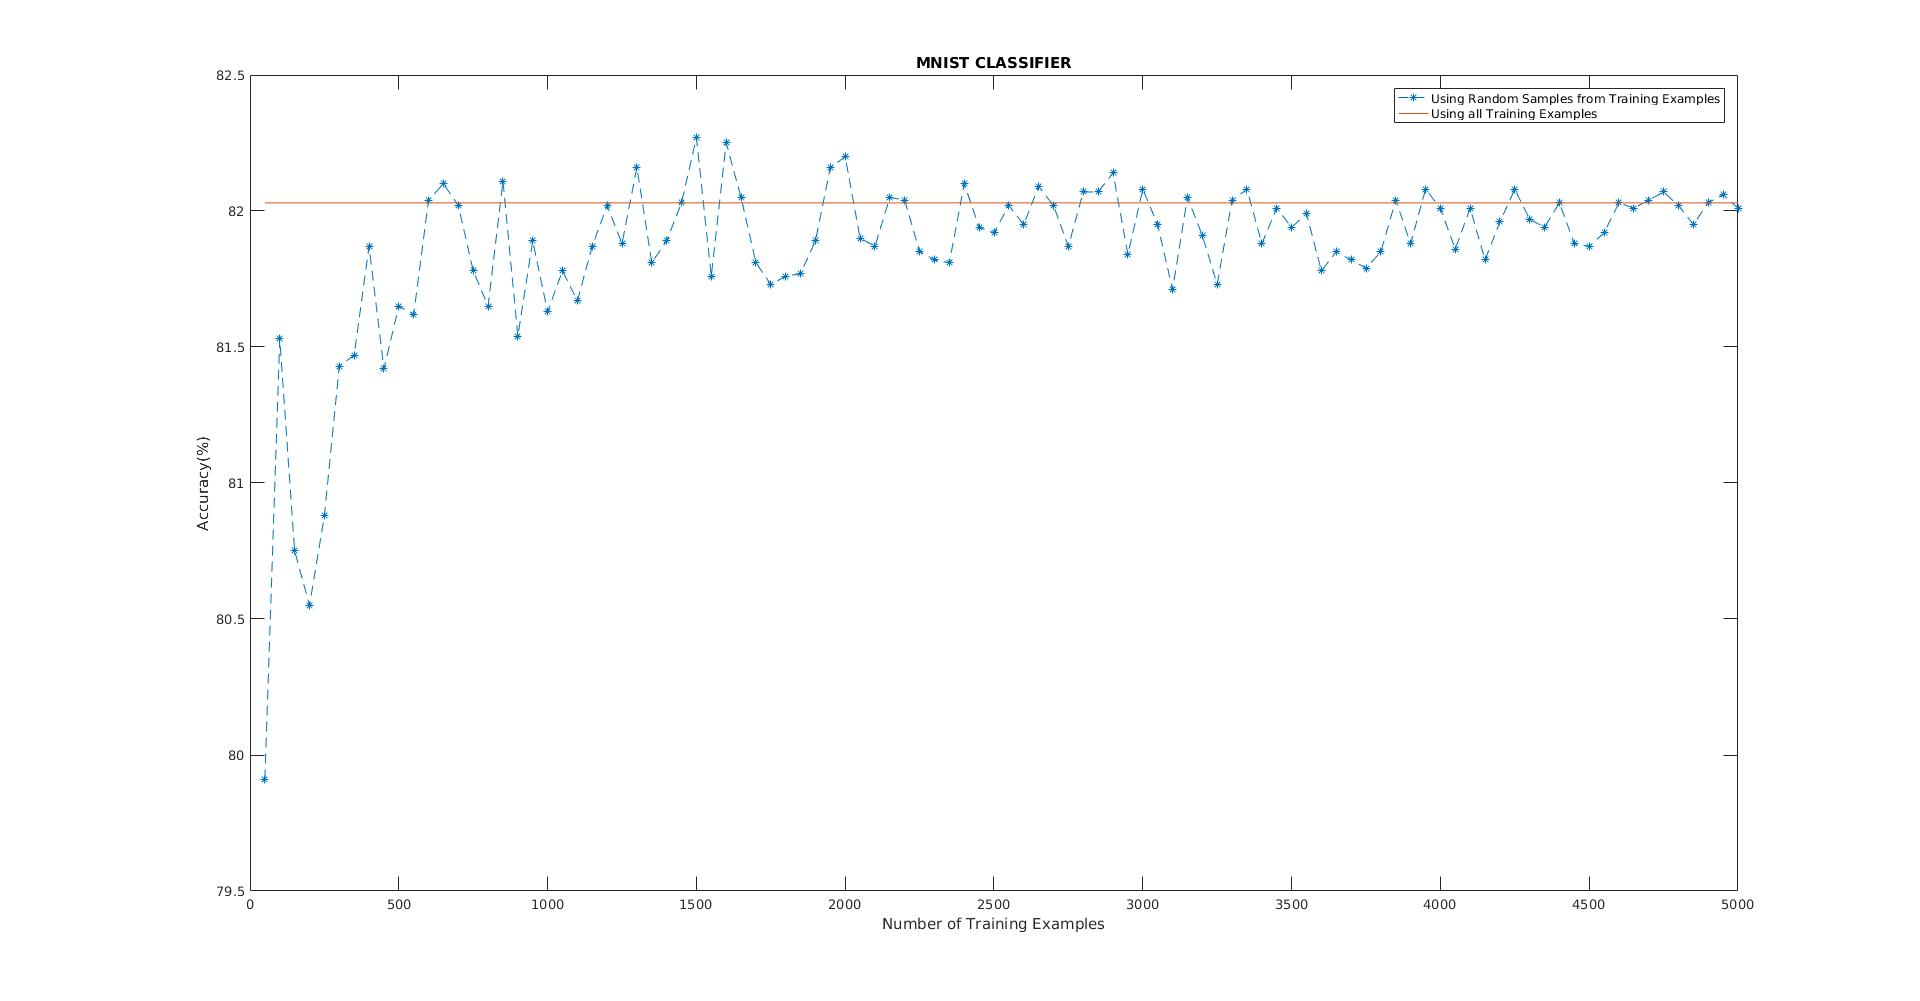
\includegraphics[width=1.12\columnwidth]{mnist_plot5.jpg}
\caption{MNIST Classifier : Accuracy vs Number of Training Examples}
\label{fig:one}
\end{figure}

Initially, when we start with just 50 training examples, the mean calculated is not able to represent the data in a most suitable way. But as we increase the number of training examples, the accuracy quickly reaches close to 82\%. Thereafter, the accuracy more or less remains the same as that when all the training examples are used. This shows that for Distance from Means Classifier, a little less number of training examples also lead to quite a good prediction for mean. This happens because more number of training examples do not have great impact on the means, since more examples would more or less lie around the same region. 


\end{document}


